\documentclass[french]{article}
\usepackage[T1]{fontenc}
\usepackage[utf8]{inputenc}
\usepackage{lmodern}
\usepackage[a4paper]{geometry}
\usepackage{babel}
\usepackage{graphicx}
\graphicspath{ {./images/} }

\usepackage{tikz}
\usetikzlibrary{calc,trees,positioning,arrows,chains,shapes.geometric,%
	decorations.pathreplacing,decorations.pathmorphing,shapes,%
	matrix,shapes.symbols,fit,arrows.meta,backgrounds}

\begin{document}
\title{Étude sur l'application de joueurs artificiels sur un jeu de stratégie en temps réel}
\author{Dimitri \bsc{Cocheril-Crèvecœur}}
\date{2023-2024}
	
\maketitle
	
\tableofcontents

\section{Introduction}
%TODO
\section{Moteur de jeu}
\subsection{Architecture}
\begin{center}
	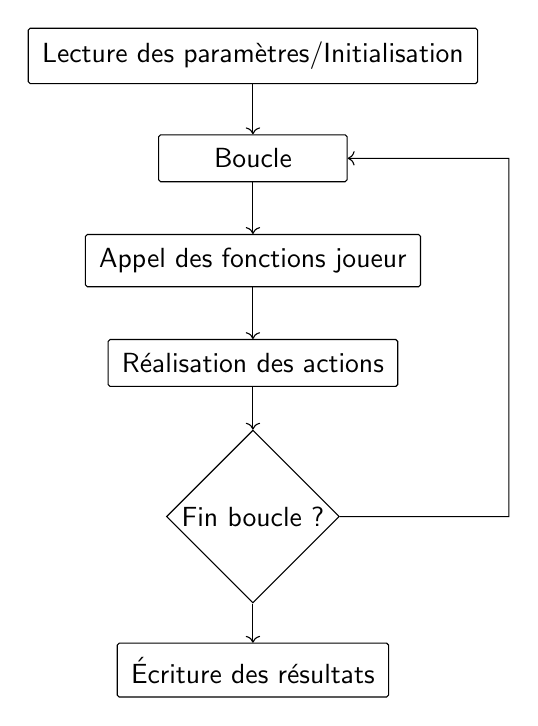
\begin{tikzpicture}[xscale=1.3,yscale=1.3, ->, every node/.style={draw, rounded corners=0.7, fill=white, font=\sffamily}, align=center, inner sep=5pt]
		\node (0) at (0,0) {Lecture des paramètres/Initialisation};
		\node [inner xsep=20pt](1) at (0,-1) {Boucle};
		\node (2) at (0,-2) {Appel des fonctions joueur};
		\node (3) at (0,-3) {Réalisation des actions};
		\node [diamond, inner sep=1pt, rounded corners=0] (4) at (0,-4.5) {Fin boucle ?};
		\node (5) at (0,-6) {Écriture des résultats};
		
		\draw (0) -> (1);
		\draw (1) -> (2);
		\draw (2) -> (3);
		\draw (3) -> (4);
		\draw (4) -> (5);
		\draw (4) -- +(2.5,0) -- +(2.5,3.5) -- (1);
		
	\end{tikzpicture}
\end{center}
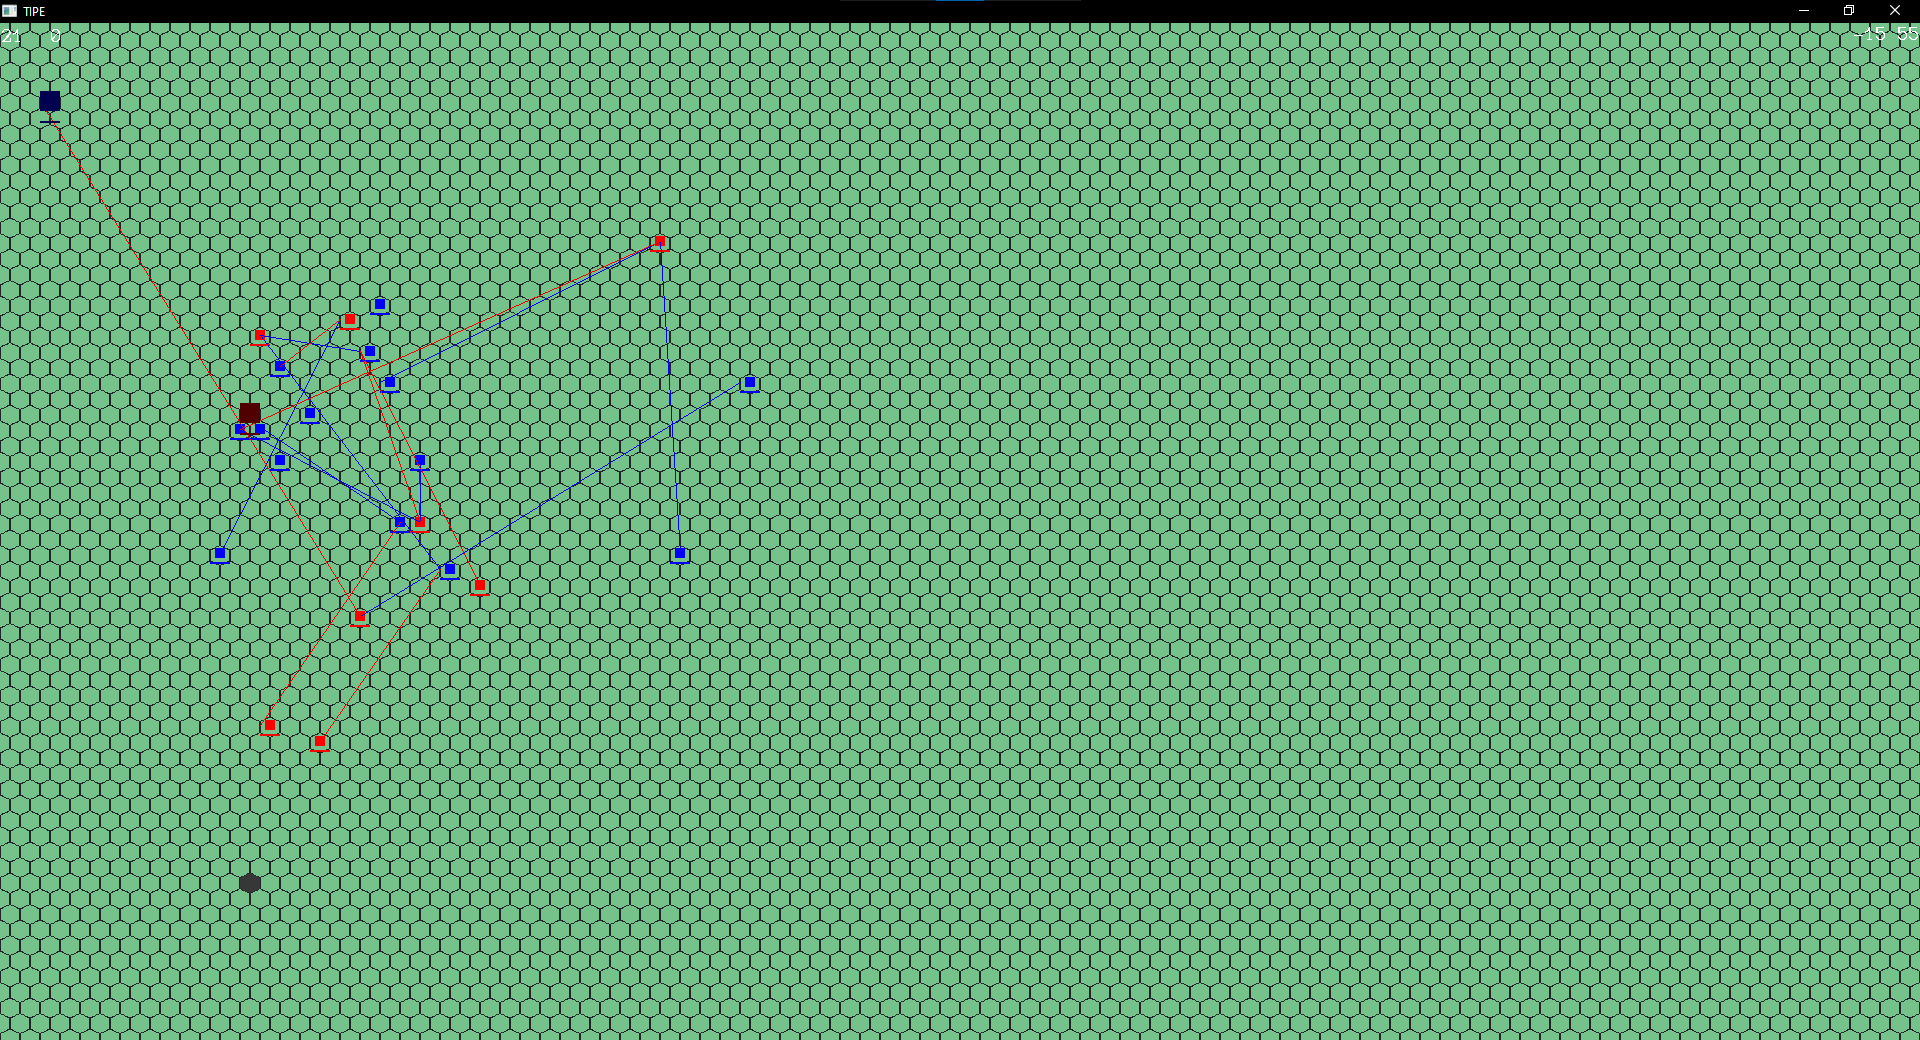
\includegraphics[width=\textwidth]{screen.png}
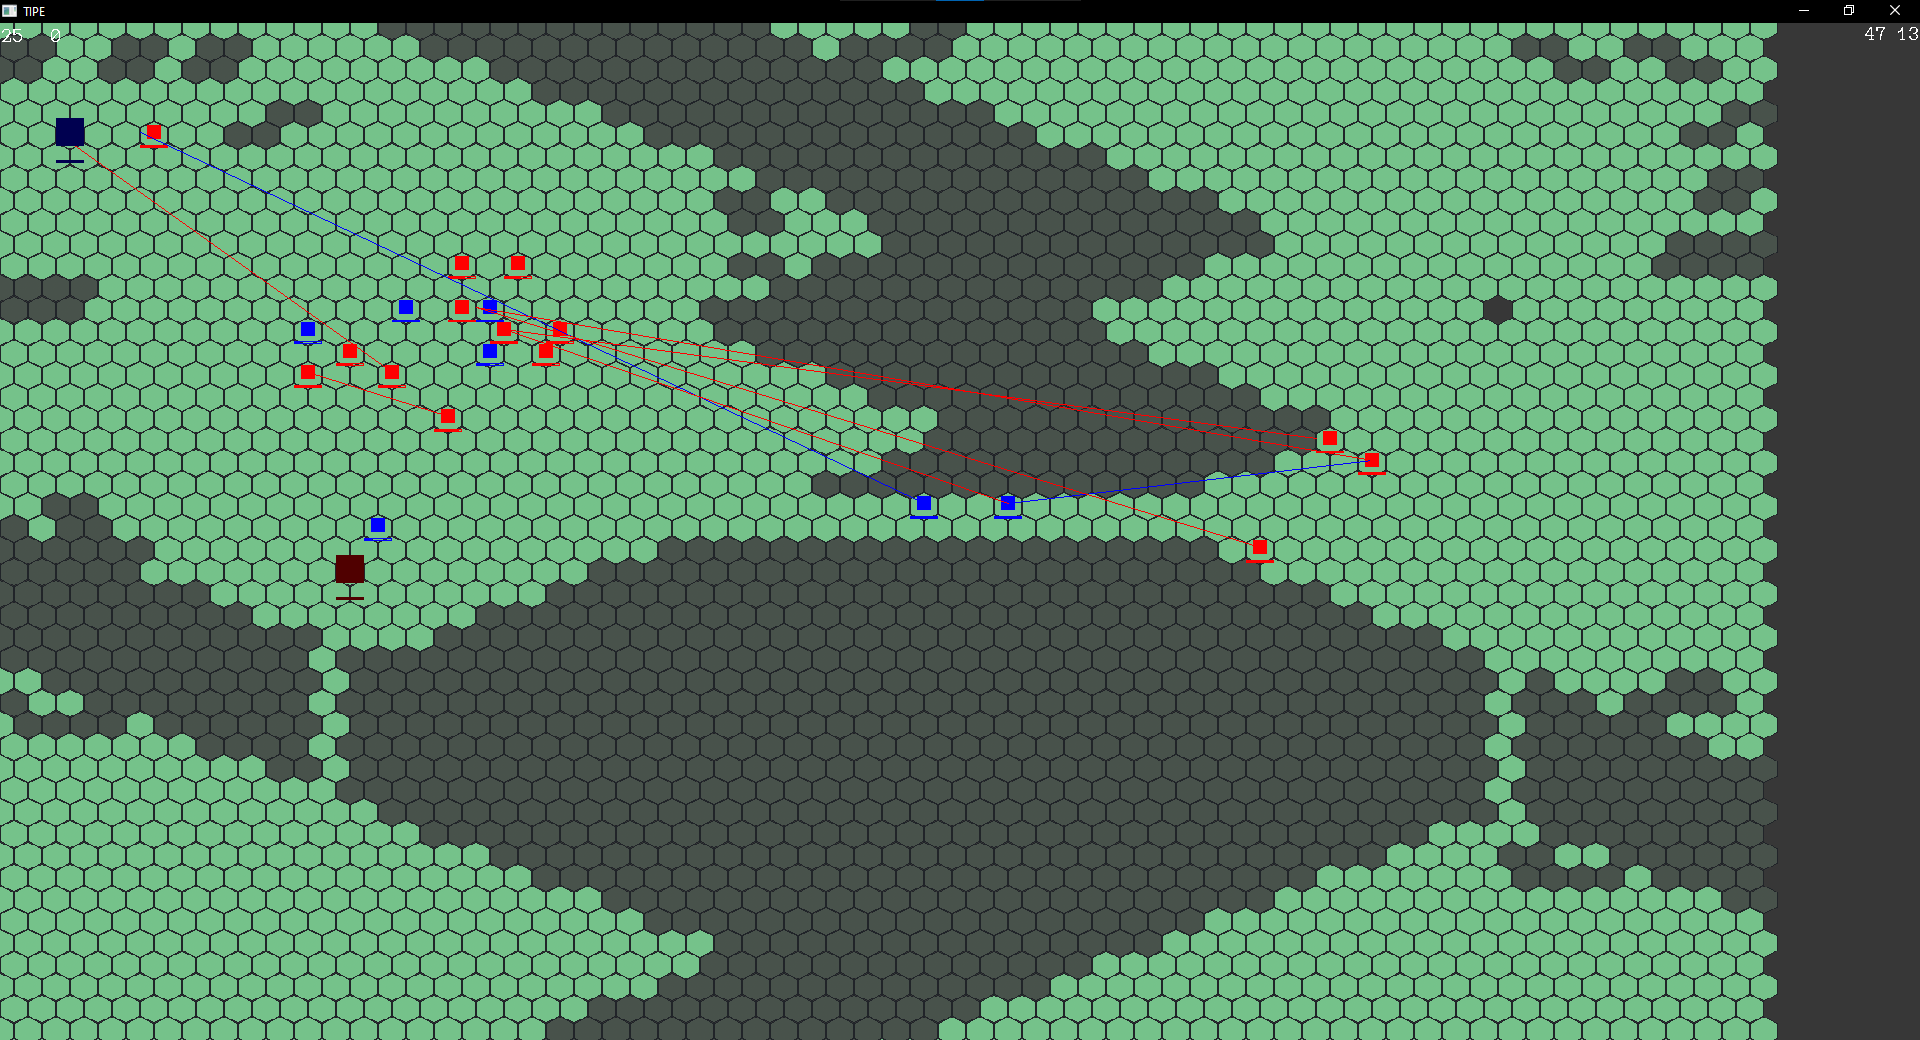
\includegraphics[width=\textwidth]{screen2.png}
\subsection{A-star}

\section{Joueur aléatoire}
\section{Joueur MCTS}
\subsection{Principe}
%TODO
\subsection{Implémentations}
%TODO
\subsection{Résultats}
%TODO
\section{Joueur "DPF"}
\subsection{Principe}
%TODO
\subsection{DB-Scan}
%TODO
\end{document}
